\documentclass{book}
\usepackage{graphicx}
\usepackage[english]{babel}
\usepackage{amsthm}
\usepackage{amsmath}
\usepackage{amssymb}
\usepackage{amsfonts}
\usepackage{physics}
\usepackage{tikz}
\usepackage[a4paper, margin=1in]{geometry}
\geometry{a4paper, margin=1in}
\usepackage{xcolor}
\graphicspath{ {./images/} }
\usepackage{svg}
\usepackage{bm}
\renewcommand{\cleardoublepage}{\clearpage}
\usetikzlibrary{decorations.markings,intersections,calc}
\usepackage{ifthen}
\usepackage{bm}
\usepackage{tikz,pgfplots}
\usepackage{etoolbox}
\usepackage{xcolor}
\tikzset{>=latex} % for LaTeX arrow head
\usepackage{xcolor}
\usepackage{appendix}
\usetikzlibrary{3d}
\usetikzlibrary{patterns}
\usetikzlibrary{patterns.meta}
\usetikzlibrary{arrows.meta,
	decorations.markings
}
\usetikzlibrary{calc}
\colorlet{force}{orange!80!black}
\tikzstyle{charge}=[thin,top color=red!50,bottom color=red!70,shading angle=20]
\tikzstyle{charge+}=[thin,top color=red!50,bottom color=red!90!black,shading angle=20]
\tikzstyle{charge-}=[thin,top color=blue!50,bottom color=blue!80,shading angle=20]
\tikzstyle{force}=[->,very thick,orange!80!black]
\tikzstyle{vector}=[->,very thick,green!45!black]
\def\a{2.5}
\def\R{0.33}
\def\F{1.8}
\pgfplotsset{compat=1.18} 
\usepackage{tikz-3dplot}
\usepackage[outline]{contour} % glow around text
\usetikzlibrary{angles,quotes} % for pic (angle labels)
\usetikzlibrary{arrows,arrows.meta}
\usetikzlibrary{calc}
\usetikzlibrary{decorations.markings}
\tikzset{>=latex} % for LaTeX arrow head

\colorlet{veccol}{green!45!black}
\colorlet{Bcol}{violet!90}
\colorlet{BFcol}{red!70!black}
\colorlet{veccol}{green!45!black}
\colorlet{Icol}{blue!70!black}
\colorlet{Ampcol}{green!60!black!70}
\tikzstyle{BField}=[->,thick,Bcol]
\tikzstyle{current}=[->,Icol,thick]
\tikzstyle{force}=[->,thick,BFcol]
\tikzstyle{vector}=[->,thick,veccol]
\tikzstyle{velocity}=[->,very thick,vcol]
\tikzstyle{charge+}=[very thin,draw=black,top color=red!50,bottom color=red!90!black,shading angle=20,circle,inner sep=0.5]
\tikzstyle{charge-}=[very thin,draw=black,top color=blue!50,bottom color=blue!80,shading angle=20,circle,inner sep=0.5]
\tikzstyle{metal}=[line width=0.3,top color=black!15,bottom color=black!25,middle color=black!20,shading angle=10]
\tikzstyle{darkmetal}=[line width=0.4,top color=red!20!black!40,bottom color=red!20!black!70,middle color=red!20!black!30,shading angle=10]
\tikzstyle{measline}=[{Latex[length=3]}-{Latex[length=3]}]
\tikzset{
  BFieldLine/.style={thick,Bcol,decoration={markings,mark=at position #1 with {\arrow{latex}}},
                                 postaction={decorate}},
  BFieldLine/.default=0.5,
  Ampcurve/.style={thick,Ampcol,decoration={markings,mark=at position #1 with {\arrow{latex}}},
                                postaction={decorate}},
  Ampcurve/.default=0.55,
  pics/Bin/.style={
    code={
      \def\R{0.12}
      \draw[pic actions,line width=0.6,#1,fill=white] % ,thick
        (0,0) circle (\R) (-135:.75*\R) -- (45:.75*\R) (-45:.75*\R) -- (135:.75*\R);
  }},
  pics/Bout/.style={
    code={
      \def\R{0.12}
      \draw[pic actions,line width=0.6,#1,fill=white] (0,0) circle (\R);
      \fill[pic actions,#1] (0,0) circle (0.3*\R);
  }},
  pics/Bin/.default=Bcol,
  pics/Bout/.default=Bcol,
}
\tikzstyle{measure}=[fill=white,midway,outer sep=2]
\contourlength{1.4pt}

% RING SHADING
\makeatletter
\pgfdeclareradialshading[tikz@ball]{ring}{\pgfpoint{0cm}{0cm}}%
{rgb(0cm)=(1,1,1);
rgb(0.719cm)=(1,1,1);
color(0.72cm)=(tikz@ball);
rgb(0.9cm)=(1,1,1)}
\tikzoption{ring color}{\pgfutil@colorlet{tikz@ball}{#1}\def\tikz@shading{ring}\tikz@addmode{\tikz@mode@shadetrue}}
\makeatother


\newtheorem*{definition}{Definition}
\newtheorem*{theorem}{Theorem}

\title{Electricity and Magnetism}
\author{Dominik Szablonski}

\begin{document}

\maketitle

\tableofcontents

\chapter{Electrostatics}
\section{Electric Charges and Coulomb's Law}
Electric charge is a physical property of matter, analogous to mass. They have 4 key properties:
\begin{enumerate}
    \item Charges come in \textbf{2 types}, + and -. Opposite charges attract, negaitve charges repel. 
    \item Charges are \textbf{quantised}. Charges are always integer number of electron charges (apart from quarks).
    \item Charge is a \textbf{conserved property}. It is conserved in a closed system.
    \item Charge is \textbf{Lorentz invariant}. A charged particle will not change its charge when moving at relativistic speed. 
\end{enumerate}
Charges follow Coulomb's law, which describes the forces between 2 charges. Consider $q_1$ and $q_2$,

\begin{figure}[h]
    \centering
    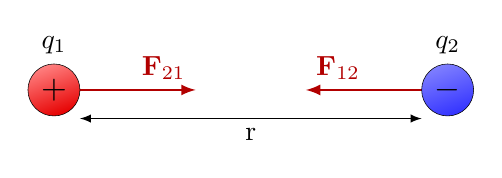
\begin{tikzpicture}
  \def\a{2.5}
  \coordinate (L) at (-\a,0);
  \coordinate (R) at (+\a,0);
    
  % FORCES
  \draw[force] (L) --++ (+\F,0) node[above left] {$\mathbf{F}_{21}$};
  \draw[force] (R) --++ (-\F,0) node[above right] {$\mathbf{F}_{12}$};
  
  % CHARGES
  \draw[charge+] (L) circle (\R) node[scale=1.2] {$+$};
  \draw[charge-] (R) circle (\R) node[scale=1.2] {$-$};
  \draw[<->]     (L)++(\R,-1.1*\R) --++ (2*\a-2*\R,0) node[midway,below] {r};
  \node[above] at (-\a,\R) {$q_1$};
  \node[above] at (+\a,\R) {$q_2$};
  
\end{tikzpicture}

    \caption{The forces of 2 unlike charges.}
    \label{fig:unlikecharges}
\end{figure}
    % ATTRACTING CHARGES

\begin{equation}
    \vb{F}_{12} = \frac{1}{4\pi\epsilon_0}\frac{q_1q_2}{r_{21}^2}\vu{r}_{21}. 
\end{equation}
$\vb{F}_{12}$ is the force acting on charge $q_2$. $\vb{r}_{21}$ is the vectorial separation of charge 1 to charge 2, i.e., $(\vb{r_2} - \vb{r_1})$, where $r_{21}$ is its magnitude and $\vu{r}_{21}$ is the unit vector. This direction will act parallel to the line joining the charges. This force also obeys Newton's third law, so $\vb{F}_{12} = -\vb{F}_{21}$. It is further important to remember that unlike charges attract, as in figure \ref{fig:unlikecharges}, and like charges repel. 
\\\\
Forces on stationary point charges follow the principle of superposition. Considering a force $\vb{F}_{21}$ on a charge, $q_1$, due to some number of charges, we can say,
\begin{equation}
    \vb{F}_{21} = \frac{1}{4\pi\epsilon_0}\sum_j\frac{q_1q_j}{r_{1j}^2}\vu{r}_{1j}.
\end{equation}
\subsection{Induced Charges}
\subsubsection{Triboelectric Effect}
This is the rubbing together of two objects to transfer electrons from one to the other. 
\subsubsection{Induced Charges Disconnected from Earth}
If a point charge comes close to a conducting body, charges of the opposite polarity within the body will moves closer to the test point charge, while the like charges will repel (one side becomes positively charged, the other negatively). However, once point charge is removed, the body will not retain its charge.
\subsubsection{Induced Charges Connected to Earth}
If a body is connected to the earth and then a point charge is placed close to it, severing the connection to earth will allow the body to retain its charge when the point charge is removed.
\subsubsection{Induced Charges on Insulators}
Bound charges can be attracted to the opposing point charge. This is called polarisation.
\section{Electric Fields}
A field is a physical quantity that has a value at all points in space and time within a system. We can consider an electric field as an area of space which exerts a certain force on a test charge, due to a distribution of charges in that area. If we say $Q$ is the test charge, then
\begin{equation}
    \vb{F_E} = Q\vb{E}
\end{equation}
and
\begin{equation}
    \vb{E} = \frac{1}{4\pi\epsilon_0}\sum_{i=1}^n\frac{q_i}{\eta^2_i}\vu*{\eta}_i,
\end{equation}
where $\vb*{\eta}$ is the vectorial separation from the $i$th charge and the point where the test charge $Q$ is located (although it does not depend on the test charge $Q$).
\subsection{Field Lines}
\begin{figure}[h]
    \centering
    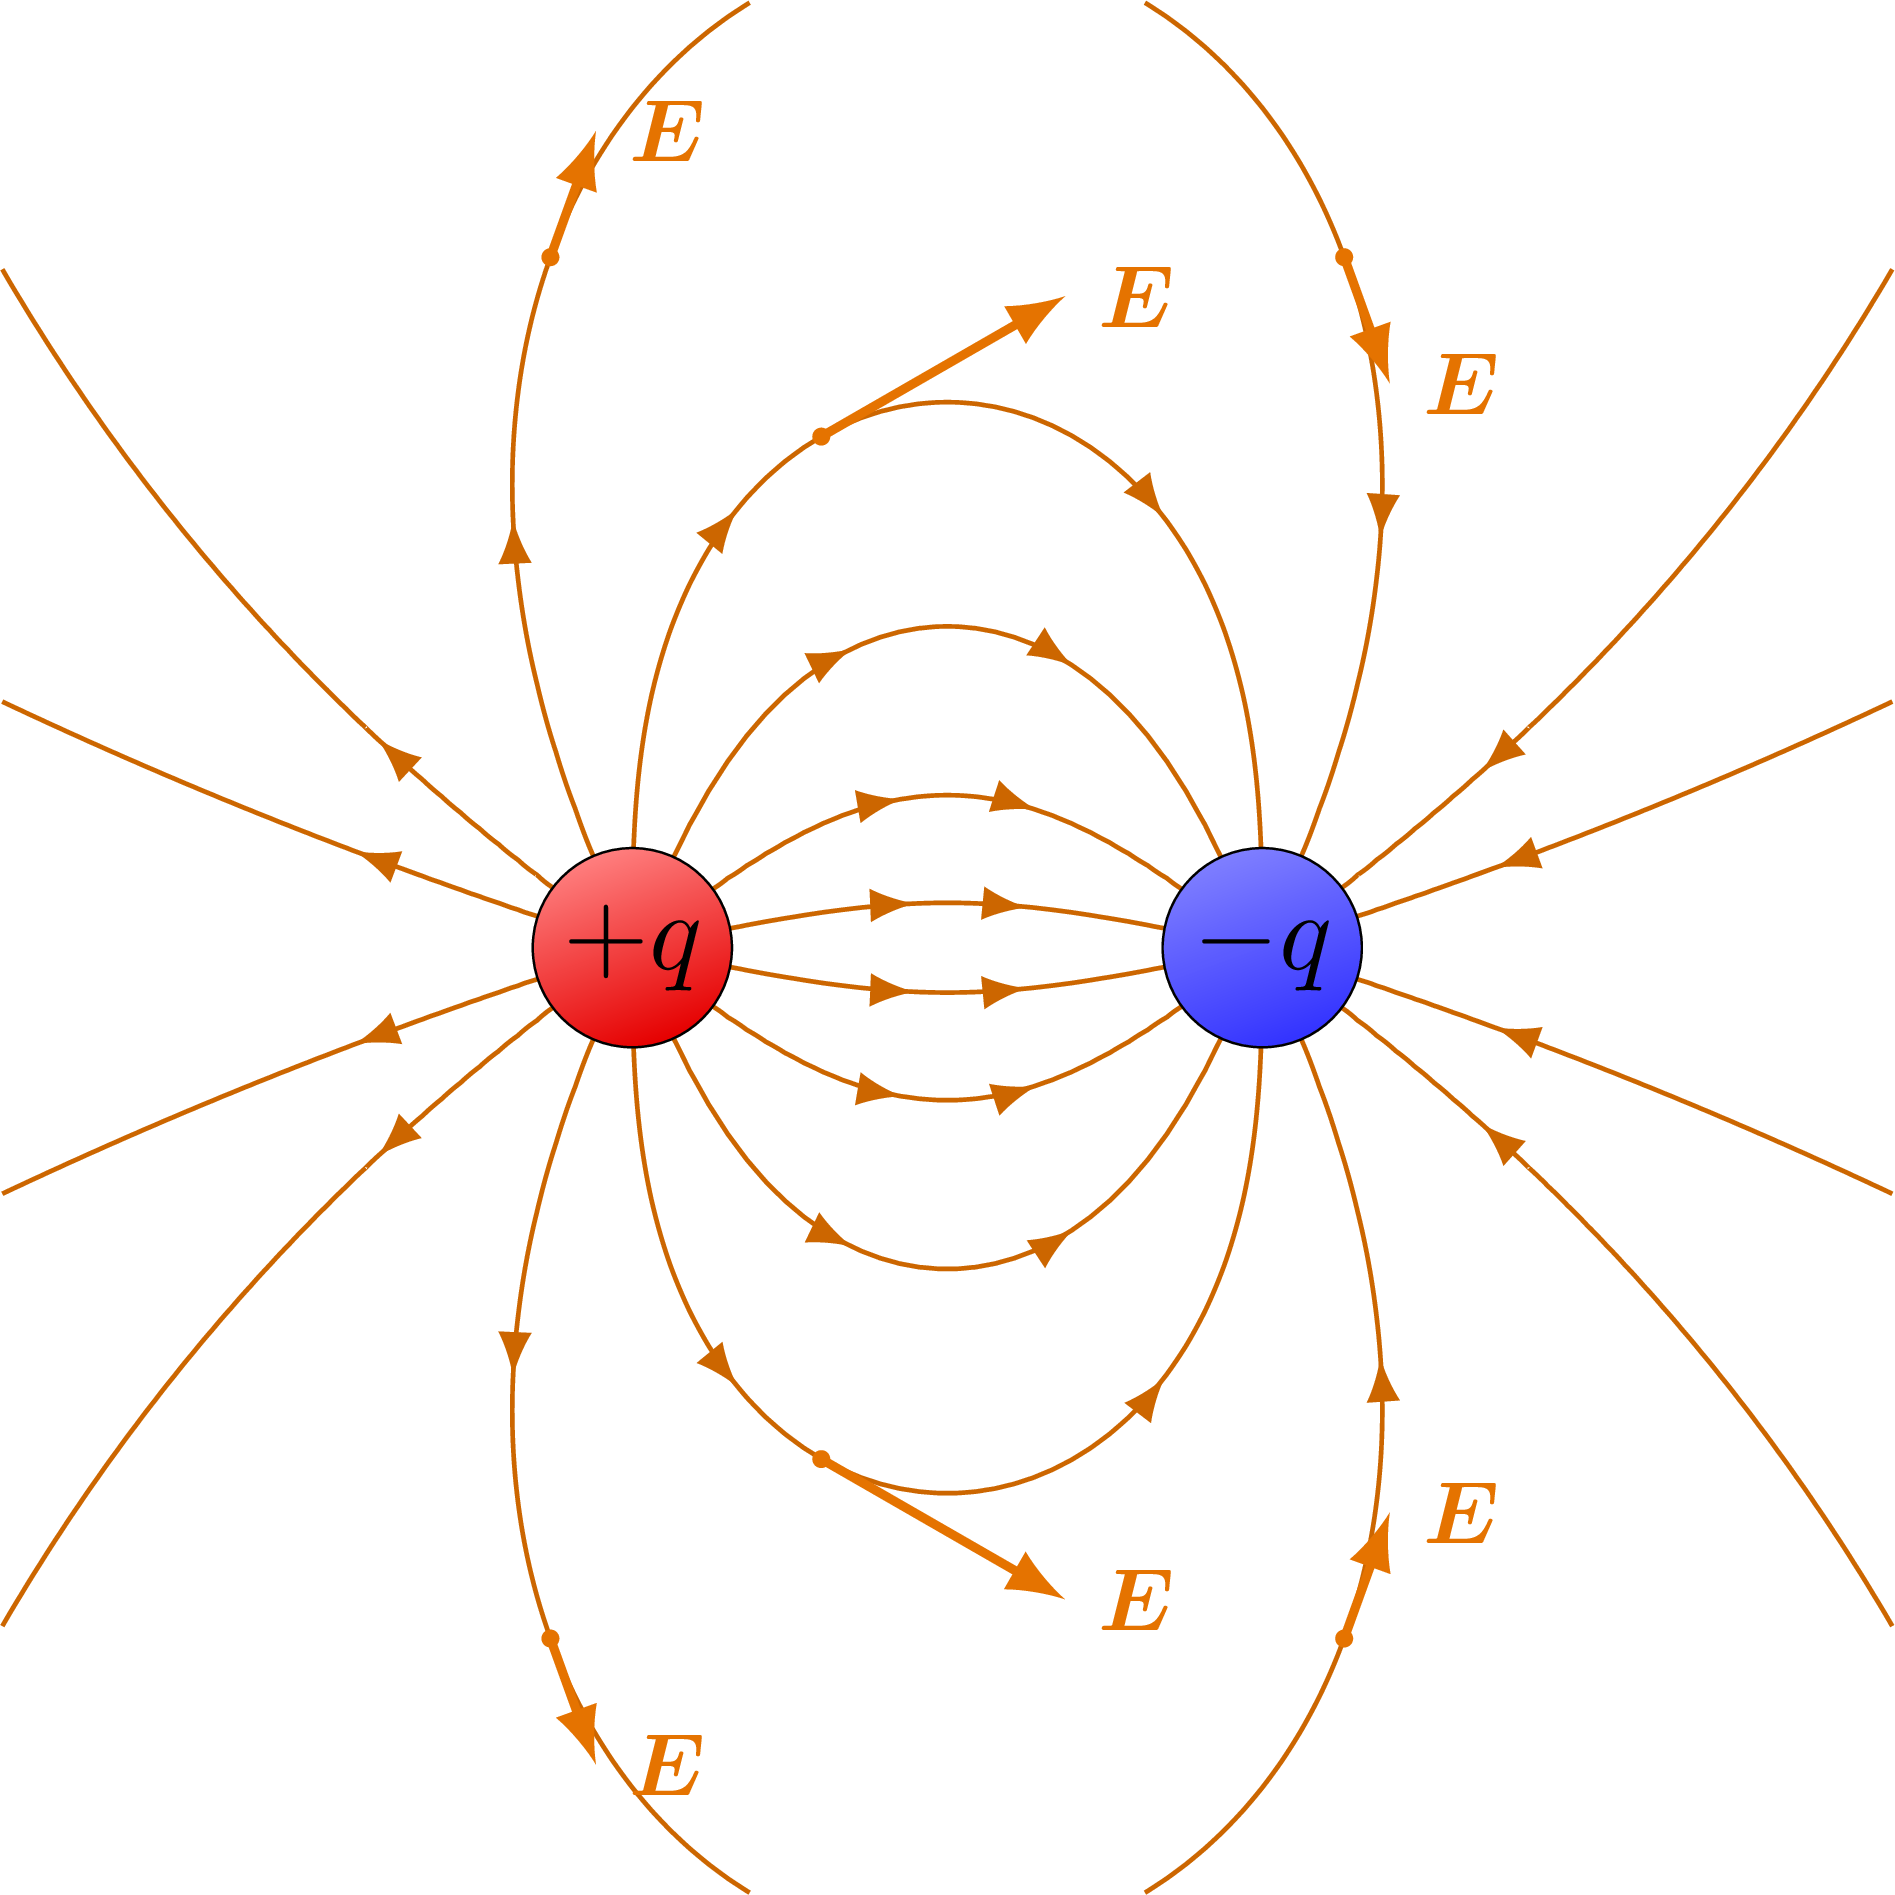
\includegraphics[width=150pt]{electric_fieldlines2-001.png}
    \caption{Electric field lines of 2 unlike point charges.}
    \label{fig:fieldlines}
\end{figure}
Figure \ref{fig:fieldlines} shows the field lines due to 2 unlike point charges. From this, we can understand some properties of field lines,
\begin{itemize}
    \item Field lines point towards negative charges,
    \item field lines either terminate on a charge or extend to infinity,
    \item and field lines never cross.
\end{itemize}
\subsection{Continuous Electric Fields}
We are able to define an electric field as,
\begin{equation}
    \vb{E}(\vb{r}) = \frac{1}{4\pi\epsilon_0}\int \frac{1}{\eta^2}\vu*{\eta}dq.
\end{equation}
The $dq$ term changes depending on the type of surface the charge is distributed against. Where $dq$ is an infinitesimal charge,
\begin{itemize}
    \item \textbf{Length} $\to$ $\lambda \dd{l}$ where $\lambda$ is the charge per unit length,
    \item \textbf{Area} $\to$ $\sigma \dd{a}$ where $\sigma$ is the charge per unit area, and $\dd{a}$ is an infinitesimal, 2-D area,
    \item \textbf{Volume} $\to$ $\rho \dd{\tau}$ where $\rho$ is the charge per unit volume, and $$\dd{\tau} = \dd{x}\dd{y}\dd{z}.$$
\end{itemize}
\subsection{Gauss' Law}
\begin{definition}
    The flux of an electric field through any closed surface is equal to the total charge within the volume enclosed by that surface divided by the permittivity of free space.
\end{definition}
As an equation,
\begin{equation}
    \oint_S \vb{E}\cdot\dd{\vb{A}} = \frac{Q}{\epsilon_0}
\end{equation}
where $Q$ is the total charge enclosed within the surface and $\dd{\vb{A}}$ is the infinitesimal area vector. It is defined,
\begin{equation}
    \dd{\vb{A}} = \dd{x}\dd{y}\vu{n}
\end{equation}
where $\vu{n}$ is the normal vector, or the vector perpendicular to the area.
\\\\
We can also write Gauss' law in vector operator form,
\begin{align}
    \div{\vb{E}} = \frac{\rho}{\epsilon_0} && \curl{\vb{E}}= 0.
\end{align}
Gauss' law will apply to all charge distributions enclosed by some surface.
\begin{figure}
    \centering
    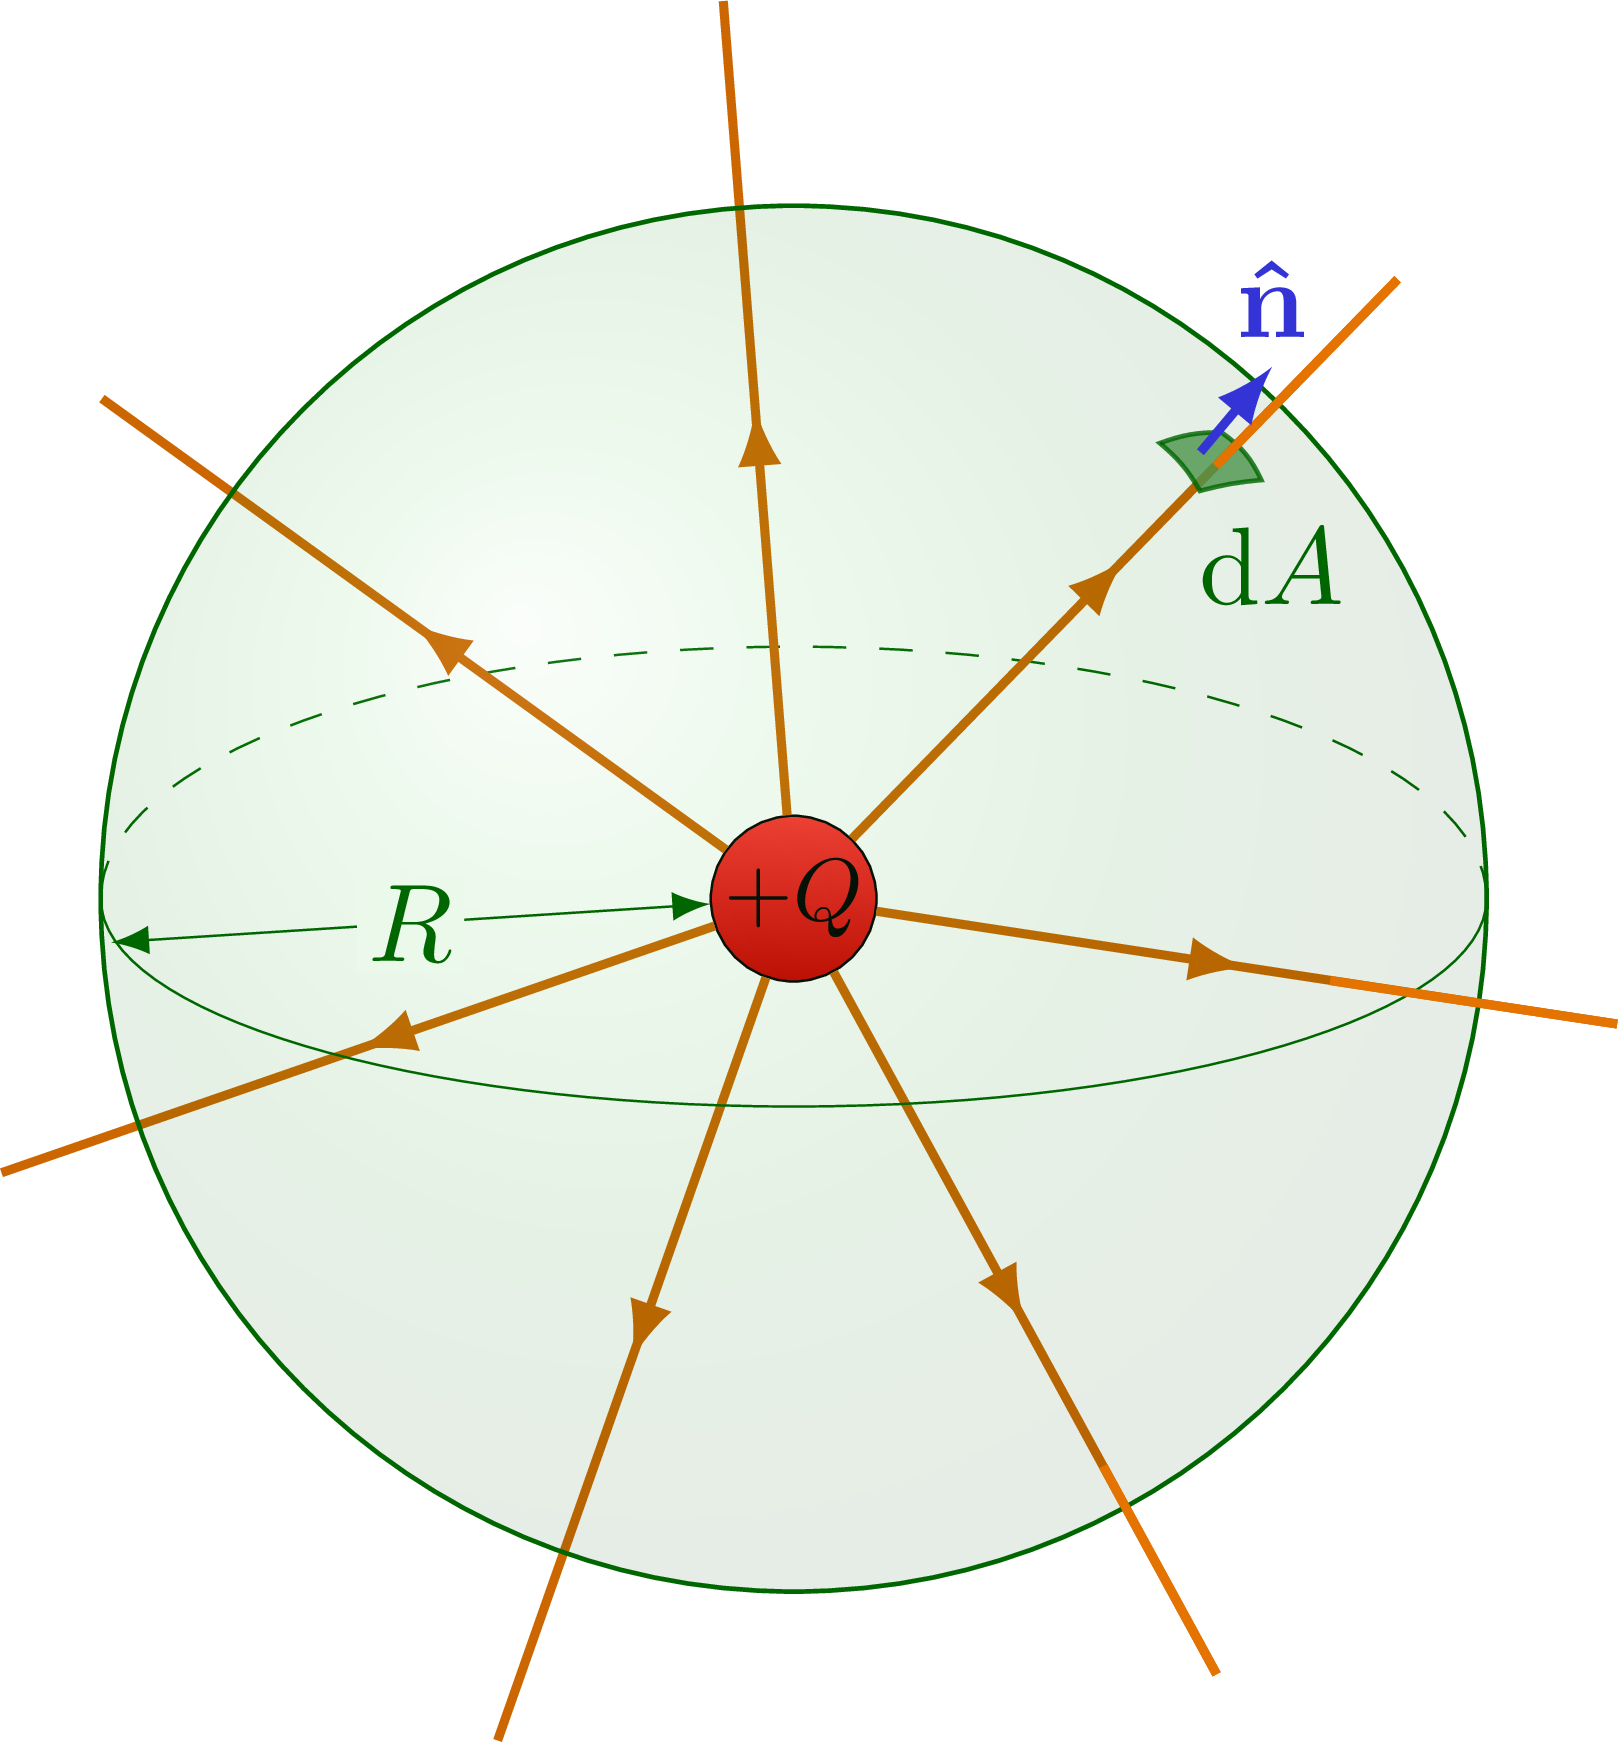
\includegraphics[width=200pt]{electric_field_sphere-001.png}
    \caption{Gauss' law visualised via a point charge within a Gaussian surface of a spherical shell.}
    \label{fig:gauss}
\end{figure}
\subsubsection{Earnshaw's Theorem}
\begin{theorem}
    It is impossible to construct an electrostatic field that will hold a charged particle in stationary equilibrium in empty space.
\end{theorem}
The proof of this theorem is by performed by contradiction. The proof below is for $q>0$.\\\\
Consider a positive charge $q$ paced at a point $\vb{z}$ within a static electric field (see figure \ref{fig:earnshaw}).
\begin{figure}
    \centering
    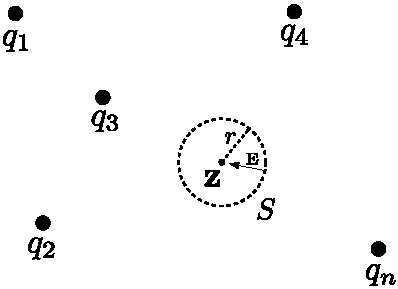
\includegraphics[width=150pt]{charges-gaussian-surface.22ec9ba7.pdf}
    \caption{A set of $n$ fixed charges and a very small Gaussian surface $S$ centered at a point $\vb{z}$.}
    \label{fig:earnshaw}
\end{figure}
For the charge to be held in stable equilibrium,
\begin{enumerate}
    \item The electric force $q\vb{E}(\vb{z})=0$, thus $\vb{E}=\vb{0}$.
    \item For a small displacement $\delta z$, $q\vb{E}(\vb{z}+\delta\vb{z})$ must point towards $\vb{z}$.
\end{enumerate}
Thus, the electrostatic force on $q$ must be restoring. Since $q>0$, $\vb{E}(\vb{z}+\delta\vb{z})$ must point towards $\vb{z}$. \\\\
Now, consider an arbitrarily small Gaussian surface $S$ enclosing the charge $q$ in the form of a spherical shell. Since $\vb{E}(\vb{x})$ points towards $q$ for any point on the surface $S$, then,
\begin{equation}
    \oint_S\vb{E}\cdot\dd{\vb{A}} = \frac{Q_{\text{enc}}}{\epsilon_0} < 0
\end{equation}
which implies there must be a negative charge enclosed within the surface $S$, contradicting the the assumption that $\vb{z}$ is a point within a vacuum.$\qed$ 
\subsection{Circulation of the electric field and electric potential}
Electric fields are conservative, so a charge moving from point $A$ to point $B$ on two different paths wil experience the same force, such that,
\begin{equation}
    \int_1 \vb{E}\cdot\dd{l} = \int_2 \vb{E}\cdot \dd{l}.
\end{equation}
Given this, we can conclude that for a charge travelling in a closed loop, the circulation is 0, given by,
\begin{equation}
    \oint_C \vb{E}\cdot\dd{l} = 0.
\end{equation}

A charge moving from $A$ to $B$ will convert electric potential to work. The electric potential $\phi$ can be defined as the potential energy per unit charge. The electric potential is a scalar field, defined at any point $\vb{r}$ as,
\begin{equation}
    \phi(\vb{r}) = -\int_{\infty}^{\vb{r}} \vb{E}\cdot d\vb{l},
\end{equation}
and the potential difference between two points, $\vb{r}_A$ and $\vb{r}_B$ as,
\begin{equation}
    \Delta\phi = \phi(\vb{r}_B) - \phi(\vb{r}_A) = \int_{\vb{r}_B}^{\vb{r}_A}\vb{E}\cdot d\vb{l}.\label{potdiff}
\end{equation}
\subsubsection{Equipotential Surfaces}
This is and area in space where the potential is the same at all points. The electric field lines are normal to the equipotential. We are able to obtain the electric field from the potential by introducing the gradient operator, $\grad$,
\begin{equation}
    \grad = \left(\pdv{}{r_i}\vb{e}_i\right).
\end{equation}
The electric field is then given by,
\begin{equation}
    \vb{E} = \grad \phi.
\end{equation}
\subsubsection{Poisson's Equation}
\begin{equation}
    \nabla^2\phi = 0.
\end{equation}
\subsection{Energy in and Electric Field}
In order to discuss the energy due to an electric field we will use the example of a parallel plate capacitor, which we discuss in a further section. We will add infinitesimal charges, $\dd{q}$ to the capacitor until it reaches a charge $Q$. Adding a charge requires work, such that,
\begin{equation}
    \dd{W} = \phi \dd{q}.
\end{equation}
This is the work stored by the electric field. We understand that $\phi$ is a function of $q$, such that $\phi = \frac{q}{C}$, thus we have,
\begin{equation}
    U = W = \int_0^Q \phi \dd{q} = \int_0^Q\frac{q}{C}\dd{q} = \frac{Q^2}{2C} = \frac{C\phi^2}{2}.
\end{equation}
We understand that for a parallel plate capacitor, 
\begin{equation}
    C = \frac{\epsilon_0A}{d}
\end{equation}
and
\begin{equation}
    \phi = Ed.
\end{equation}
Thus,
\begin{equation}
    U = \frac{\epsilon_0A(Ed)^2}{2d}.
\end{equation}
Thus, the potential energy depends on the electric field strength. We can say generally, for all charge distributions, the energy density $u$ stored by a general electric field of magnitude $E$ is,
\begin{equation}
    u = \frac{\epsilon_0E^2}{2}.
\end{equation}
We also have that, generally, the total work done by a continous charge distribution is,
\begin{equation}
    W = \frac{\epsilon_0}{2}\int_{\text{all space}} E^2 \dd{V}.
\end{equation}
\section{Conductors and Capacitors}
A perfect conductor meets the following conditions:
\begin{itemize}
    \item It has no resistance.
    \item All points on and in the conductor are equipotential.
    \item $\vb{E} = 0$ inside, $\implies \rho = 0$.
\end{itemize}
\begin{proof}
    Suppose a perfect conductor. We will suppose that there is an electric field between the points $A$ and $B$ (see figure \ref{fig:cond}).
    \begin{figure}[h]
        \centering
        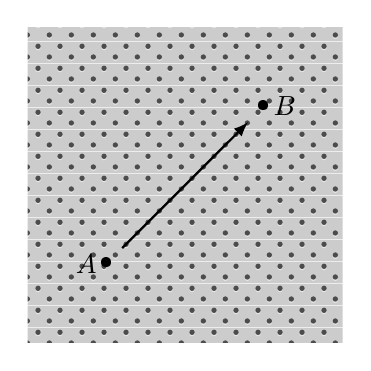
\begin{tikzpicture}
            \fill[pattern=crosshatch dots gray] (-1,-1) rectangle (3,3);
            \node (A) at (0,0) {\textbullet};
            \node (B) at (2,2) {\textbullet};
            \node[anchor = east] at (A) {$A$};
            \node[anchor = west] at (B) {$B$};
            \draw[->,thick] (A) -- (B);
        \end{tikzpicture}
        \caption{}
        \label{fig:cond}
    \end{figure}
    \\
    Since this is a perfect conductor, the resistance, $R = 0$. Let us now consider the potential inside this conductor, along the line of this electric field,
    \begin{equation*}
        \Delta\phi = \int \vb{E}\cdot\dd{\vb{l}} = \int E\dd{l} = +\text{ive}.
    \end{equation*}
    However, by Ohm's law,
    \begin{equation}
        \Delta\phi = IR.
    \end{equation}
    $R=0$, and $\Delta\phi$ is $+$ive, this implies an infinite current running through the conductor. This cannot be true, and is a contradiction, therefore
    $$\Delta\phi = 0 \implies \vb{E} = 0,$$
    by Gauss' law. 
\end{proof}
\noindent
Further, \textbf{all excess charge will lie at the surface of the conductor}.
\begin{proof}
    Consider a perfect spherical conductor of some radius, and a Gaussian sphere inside the conductor.  
    \begin{figure}
        \centering
        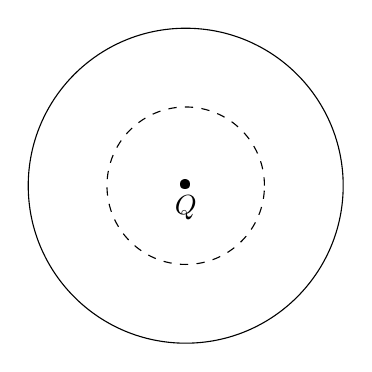
\begin{tikzpicture}
            \node (C) at (0,0) {\textbullet};
            \draw[] (C) circle (2);
            \draw[dashed] (C) circle (1);
            \node[anchor = north] at (C) {$Q$};
        \end{tikzpicture}
        \caption{}
        \label{fig:equipotential}
    \end{figure}
    \\
    Using Gauss' law,
    \begin{equation*}
        \vb{E}\cdot\dd{\vb{A}} = \frac{Q_{\text{enc}}}{\epsilon_0},
    \end{equation*}
    however, $\vb{E} = 0$,
    $$\implies Q_{\text{enc}} = 0,$$
    so we can naturally conclude that all charge must lie on the surface on the conductor.
\end{proof}\noindent
Naturally, the conductor being equipotential naturally follows as there are no unbalanced charges within the conductor.
\subsection{Faraday Cages}
A Faraday cage is a conductor with cavity, where external electric fields \textbf{do not} effect the electric field inside the cavity. \\\\
The reasoning behind this is that the free electrons in the conductor can rearrange themselves so that the electric field inside the conductor remains at 0. Thus, the E-flied in the cavity should also be 0. However, we can provide a more rigorous proof by contradiction.
\begin{proof}
    We will consider setup like in figure \ref{fig:cond2}. We will bring a +ve charge close to the conductor. Charges will be induced on the external surface of the conductor. However, by Gauss' law, if we consider a Gaussian surface through the conductor, surrounding the entire cavity, we will find that the total charge is 0. 
\begin{figure}[h]
        \centering
        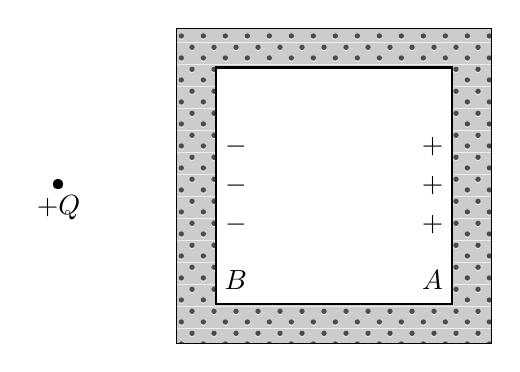
\begin{tikzpicture}
            \filldraw[pattern=crosshatch dots gray] (-1,-1) rectangle (3,3);
            \filldraw[color=black,thick,fill=white] (-0.5,-0.5) rectangle (2.5,2.5);
            \node (A) at (-0.25,-0.2) {$B$};
            \node (B) at (2.25,-0.2) {$A$};
            \node at (-0.25, 1) {$-$};
            \node at (-0.25, 1.5) {$-$};
            \node at (-0.25, 0.5) {$-$};
            \node at (2.25, 1) {$+$}; 
            \node at (2.25, 0.5) {$+$}; 
            \node at (2.25, 1.5) {$+$}; 
            \node (Q) at (-2.5,1) {\textbullet};
            \node[anchor=north] at (Q) {$+Q$};
        \end{tikzpicture}
        \caption{}
        \label{fig:cond2}
    \end{figure}
This may lead us to believe that charges were induced on on the inner surface of the conductor, however, this cannot be true. Let us consider the circulation of the electric field. We will assume that there is an electric field running from $A$ to $B$. We will setup our integral such that our line runs from $B \to A \to B$, such that $A \to B$ runs through the conductor, and $B \to A$ runs along the electric field lines. We know,
\begin{equation}
    \int_{B\to A}\vb{E}\cdot\dd{\vb{l}} = 0.
\end{equation}
We also know the circulation through a conductor is 0, so,
\begin{equation}
    \oint \vb{E}\cdot \dd{\vb{l}} = 0 = \int_{A \to B} \vb{E}\cdot\dd{\vb{l}} + \int_{B \to A}\vb{E}
\cdot\dd{\vb{l}} = \int_{A\to B}\vb{E} \cdot \dd{\vb{l}} = 0\end{equation}
We can then conclude,
\begin{equation}
    E_{A\to B} = E_{\text{cavity}} = 0 
\end{equation}
this implies that there cannot be charges on the inner surface.
\end{proof}
\subsubsection{Charge Inside Faraday Cage}
If we place a charge inside of a Faraday cage, it will induce charges on the inner surface, so that the total charge enclosed by within the conductor is 0. However, this will also induce charges on the outer surface of the conductor, producing an electric field.
\begin{figure}[h]
        \centering
        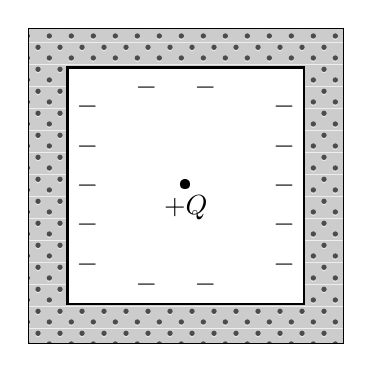
\begin{tikzpicture}
            \filldraw[pattern=crosshatch dots gray] (-1,-1) rectangle (3,3);
            \filldraw[color=black,thick,fill=white] (-0.5,-0.5) rectangle (2.5,2.5);
            \node (A) at (-0.25,0) {$-$};
            \node (B) at (2.25,0) {$-$};
            \node at (-0.25, 1) {$-$};
            \node at (-0.25, 1.5) {$-$};
            \node at (-0.25, 0.5) {$-$};
            \node at (2.25, 1) {$-$}; 
            \node at (2.25, 0.5) {$-$}; 
            \node at (2.25, 1.5) {$-$}; 
            \node at (2.25, 2) {$-$};
            \node at (-0.25, 2) {$-$};
            \node at (0.5,2.25) {$-$};
            \node at (1.25,2.25) {$-$};
            \node at (0.5,-0.25) {$-$};
            \node at (1.25,-0.25) {$-$};
            \node (Q) at (1,1) {\textbullet};
            \node[anchor=north] at (Q) {$+Q$};
        \end{tikzpicture}
        \caption{}
        \label{fig:cond3}
    \end{figure}
We will also state if a conductor has multiple cavities, charges placed within those cavities will have no effect on on charges/fields of the other cavities.
\subsection{Capacitors}
\begin{figure}[h]
    \centering
    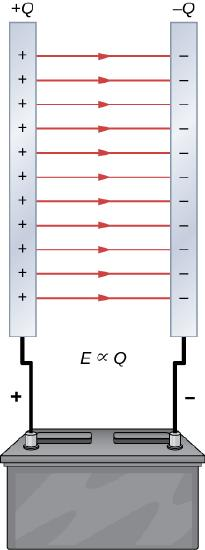
\includegraphics[height=250pt]{CNX_UPhysics_25_01_Electric.jpg}
    \caption{Electric field due to a parallel plate capacitor}
    \label{fig:capacitor}
\end{figure}
\noindent Capacitors are able to store charge when they are connected to potential. Since $\Delta \phi \propto Q$, we can introduce a capacitance $C$,
\begin{equation}
    Q = C\Delta \phi. \label{capacitance}
\end{equation}
In order to find the capacitance of a capacitor, we must combine Gauss' law in order to find the electric field, along with the equation of potential difference as given by equation \eqref{potdiff}. \\\\
\textbf{NOTE:} There will only ever be an electric field present \textit{between the plates of the capacitor}. The electric field will be 0 outside the capacitor.
\section{Dipoles}
\begin{figure}[h]
    \centering
    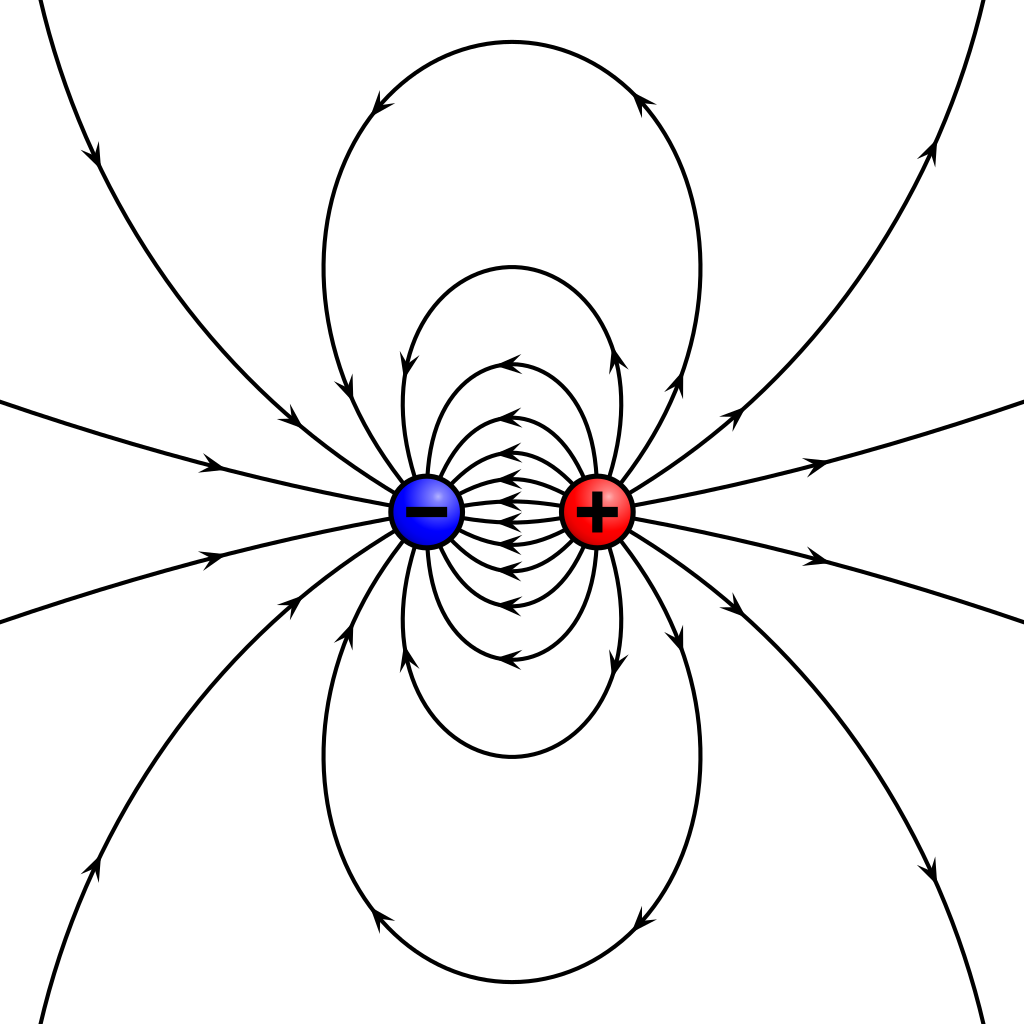
\includegraphics[width=100pt]{VFPt_dipole_electric.svg.png}
    \caption{Electric field due to 2 dipoles.}
    \label{fig:dipoles}
\end{figure}
Electric dipoles are 2 equal and opposite charges which are separated from each other by a small distance. Let's call this vectorial separation $\vb{d}$. We can then define the moment of the electric dipole as,
\begin{equation}
    \vb{p}= q\vb{d}.
\end{equation}
\subsection{Electric field due to dipole}
First, we must consider the potential due to a dipole. We will consider some point $A$ at a separation $r$ from the centre of the dipole. We will assume that $r >> d$. Using the principle of superposition,
\begin{equation}
    \phi = \phi_+ + \phi_- = \frac{Q}{4\pi\epsilon_0 r_1} - \frac{Q}{4\pi\epsilon_0r_2}.
\end{equation}
We can then define,
\begin{equation}
    r_n = \begin{cases}
        n = 1 & r - \frac{d}{2}\cos\theta \\
        n = 2 & r + \frac{d}{2}\cos\theta
    \end{cases}.
\end{equation}
We can then find an expression for $\frac{1}{r_1}$ and $\frac{1}
{r_2}$,
\begin{equation}
    \frac{1}{r_1} = \frac{1}{r-\frac{d}{2}\cos\theta} \approx
    \frac{1 + \frac{d\cos\theta}{2r}}{r}
\end{equation}
and the expression for $\frac{1}{r_2}$ follows similarly. 
\\\\
We then get,
\begin{equation}
    \phi = \frac{Q}{4\pi\epsilon_0r}\left[\left(1 + \frac{d\cos\theta}{2r}\right)-\left(1 - \frac{d\cos\theta}{2r}\right)\right] = \frac{Qd\cos\theta}{4\pi\epsilon_0 r^2}.
\end{equation}
We can then find the general electric field due to a dipole by,
\begin{equation}
\begin{split}
    \vb{E} & = -\grad \phi = -\left(\pdv{\phi}{r}\vu{r} + \frac{1}{r}\pdv{\phi}{\theta}\vu*{\theta}\right) \\
    & = \frac{Qd}{4\pi\epsilon_0 r^3}(2\cos\theta \vu{r} + \sin\theta \vu*{\theta}).
\end{split}
\end{equation}
\subsection{Energy and Torque on Electric Dipole}
\begin{figure}
    \centering
    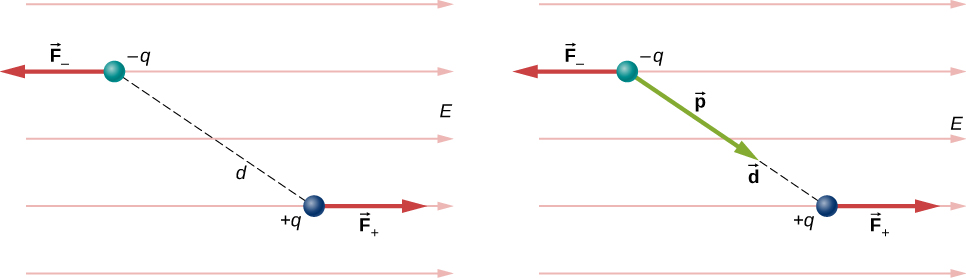
\includegraphics[width=\textwidth]{CNX_UPhysics_22_07_DipoleRot.jpg}
    \caption{A dipole
in an external electric field. (a) The net force on the dipole
is zero, but the net torque is not. As a result, the dipole
rotates, becoming aligned with the external field. (b) The dipole moment
is a convenient way to characterize this effect. The $\vb{d}$ points in the same direction as $\vb{p}$ .}
    \label{fig:diprot}
\end{figure}
If we consider a dipole in an electric field, we understand that the net force acting on it is 0. However, an angle between $\vb{p}$ and $\vb{E}$ results in the dipole experiencing a torque. \\\\
For each charge, a force $q|\vb{E}|$ acts at a perpendicular distance $\frac{d}{2}$. Using superposition,
\begin{equation}
    \vb*{\tau} = \vb*{\tau_+} + \vb*{\tau_-} = 2q|\vb{E}|\frac{d}{2}\sin\theta \vu{z} = \vb{p}\cross \vb{E}.
\end{equation}
There is then an equilibrium at $\theta = 0$, from which we can determine that the dipole attempts to align itself with the electric field. The potential is then given by,
\begin{equation}
    U = \vb{p}\cdot \vb{E}.
\end{equation}

\chapter{Magnetostatics}
The force due to a magnetic field on a moving charge is given by
\begin{equation}
    \vb{F} = q(\vb{v}\cross\vb{B}). \label{bfieldforce}
\end{equation}
The \textbf{Lorentz force} combines the force due to the electric field and the magnetic field,
\begin{equation}
    \vb{F} = q(\vb{E} + \vb{v}\cross\vb{B}).
\end{equation}
\section{Motion of a particle in a uniform B-field}
The force due to a magnetic field is always perpendicular to the velocity. Thus, for a particle with general $\vb{v}$, relative to the direction of the magnetic field, $v_{||}$ will always remain constant, whereas the $v_{\perp}$ component will cause circular motion. Thus, the particle will undergo helical motion with a radius,
\begin{equation}
    r = \frac{mv_{\perp}}{qB}.
\end{equation}

\section{Force on a current carrying wire}
Let us assume a wire of length $l$ and cross sectional area $A$. The current in the wire will be due to each charge $q$ moving with velocity $\vb{v}$. The charge density is $n$, so the total number of charges is $nAl$. Thus, the current will be,
\begin{equation}
    \vb{I} = nAq\vb{v}.
\end{equation}
\textbf{NOTE:} Positive current denotes flow of positive charge.
\\\\
Each charge experiences a force as in \eqref{bfieldforce}. Thus, the net force on the wire is,
\begin{equation}
    \vb{F}_{\text{wire}} = nAlq(\vb{v}\cross\vb{B}) = l (\vb{I}\cross \vb{B}). \label{forceonwire}
\end{equation}
\section{Work done by a magnetic field}
We understand that work is given by,
\begin{equation*}
    W = \int \vb{F}\cdot \dd{\vb{l}}.
\end{equation*}
Further, for a moving particle, we can define the infinitesimal line element as, $\dd{\vb{l}} = \vb{v}\dd{t}$. Thus, the work done by a magnetic field can be given by,
\begin{equation}
    W = \int \vb{F}_{\text{m}} \cdot \vb{v}\dd{t} = \int (\vb{v}\cross\vb{B})\cdot\vb{v}\dd{t}.
\end{equation}
Let's point out, $(\vb{v}\cross \vb{B}) \perp \vb{v} \implies (\vb{v}\cross\vb{B})\cdot\vb{v} = 0 \implies$ \textbf{Magnetic fields do \textit{no work}}.

\section{Biot-Savart Law}
This law states that moving charges create magnetic fields, such that,
\begin{equation}
    \dd{\vb{B}} = \frac{\mu_0I}{4\pi r^2}\dd{\vb{l}}\cross\vu{r}
\end{equation}
where $\dd{\vb{B}}$ is the infinitesimal magnetic field at a point $\vb{r}$ and $\dd{\vb{l}}$ is an infinitesimal length through which current runs. We can write this in vector integral form,
\begin{equation}
    \vb{B} = \frac{\mu_0}{4\pi}\int_C \frac{I\dd{\vb{l}}\cross\vu{r}}{r^2}.
\end{equation}
For examples of use see appendix B.
\section{Flux and Circulation of Magnetic Field}
Magnetic fields always form closed loops, therefore the magnetic flux of electric fields is always 0. 
\begin{align}
    &\oint_S \vb{B}\cdot\dd{\vb{A}} = 0 \implies \text{There are no magnetic monopoles} \\
    \implies & \div{\vb{B}} = 0.
\end{align}
The circulation of a magnetic field is given by Ampere's law, which applies \textit{only to magnetostatics},
\begin{equation}
    \oint \vb{B}\cdot \dd{\vb{l}} = \mu_0 I_{\text{enc}} = \mu_0\int_S \vb{J}\cdot\dd{\vb{A}}
\end{equation}
where $\vb{J}$ is the current density vector. We can write Ampere's law in differential form,
\begin{equation}
    \curl{\vb{B}} = \mu_0\vb{J}.
\end{equation}
\textbf{NOTE:} Magnetic fields follow the principle of superposition.
\subsection{Consistency with Biot-Savart law}
Let us consider a current carrying wire, whose magnetic field a distance $s$ away from the wire is,
\begin{equation}
    \vb{B}(s) = \frac{\mu_0 I}{2\pi s}\vu*{\theta}.
\end{equation}
Let us consider an Amperien loop $C$ of radius $s$ centered around the wire. The magnetic field around this loop will be constant, as we can say,
\begin{equation}
    \dd{\vb{l}} = \dd{l}\vu*{\theta} \implies \vb{B}\cdot\dd{l} = B\dd{l}.
\end{equation}
Applying Ampere's law,
\begin{equation}
    \oint \vb{B}\cdot\dd{\vb{l}} = B\oint\dd{l} = B 2\pi s = \mu_0 I,
\end{equation}
which is consistent with the Biot-Savart law.
\newpage

\section{Magnetic Dipoles}
\begin{figure}
    \centering
    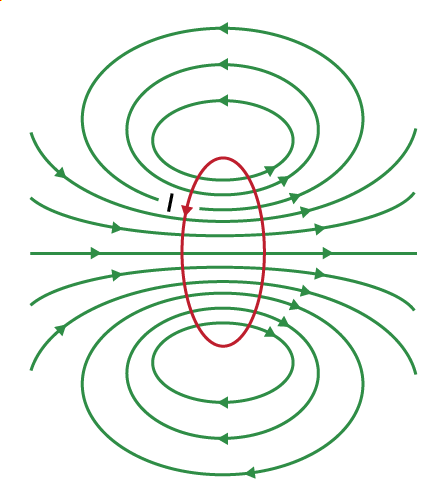
\includegraphics[height=200pt]{Magneticfieldofacurrentloop.png}
    \caption{Magnetic dipoles are the fundamental building blocks of magnetic fields, and are produced by a loop of current.}
    \label{fig:dipolefieldmagnet}
\end{figure}
Magnetic dipoles are the fundamental building blocks of magnetic fields. Dipole fields are generated by a loop of current, like in figure \ref{fig:dipolefieldmagnet}.
\subsection{Magnetic Moment}
The magnetic field due to dipole at $z >> a$, is,
\begin{equation}
    \vb{B} = \frac{\mu_0 I a^2}{2z^3}\vu{z}.
\end{equation}
We can then consider a magnetic moment, visualised by figure \ref{fig:magneticmoment}, and given by,
\begin{equation}
    \vb*{\mu} = I\vb{A}
\end{equation}
where $\vb{A}$ is the area vector of the area enclosed by the loop of current in a direction perpendicular to the loop.
\begin{figure}
    \centering
    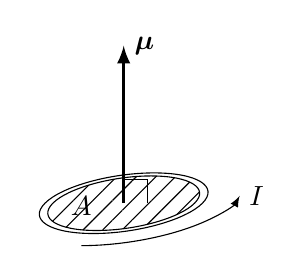
\begin{tikzpicture}
        \begin{scope}[canvas is zx plane at y = 0]
            \draw (0,0) circle (1);
            \filldraw[pattern={Lines[angle=45,distance=5pt]}] (0,0) circle (0.9);
            \node at (0.1,-0.5) {$A$};
            \draw[->] (0:1.4) arc (0:100:1.4) node[anchor=west] {$I$};
        \end{scope}
        \draw[->, very thick] (0,0,0) -- (0,2,0) node[anchor=west] {$\vb*{\mu}$};
        \draw (0,0.3,0) -- (0.3,0.3,0) -- (0.3,0,0);
        
    \end{tikzpicture}
    \caption{Visualisation of magnetic moment.}
    \label{fig:magneticmoment}
\end{figure}\\\\
Electrons have magnetic moments, if all electrons' magnetic moment points in the same direction we get a bar magnet. \\\\
We can also analyse the behaviour of magnetic dipoles in a uniform external magnetic field. This is similar to what happens when placing an electric dipole in a uniform electric field. It will experience a torque and have potential energy, given by,
\begin{align}
    \vb*{\tau} = \vb*{\mu} \cross \vb{B} && U = -\vb*{\mu} \cdot \vb{B}.
\end{align}

\chapter{Magnetodynamics}
\section{Electromotive Force}
A battery has to do work to seperate charge to overcome the electric field inside the battery. The work done per unit charge can be thought of in the terms of the force per unit charge, $\frac{\vb{F}}{q}$,
\begin{equation}
    \frac{W_{\text{battery}}}{q} = \frac{1}{q}\int_-^+ \vb{F}\cdot\dd{\vb{l}} = \phi_+ - \phi_- = \Delta \phi. \label{forceperunitchargepotential}
\end{equation}
The EMF is then the work done per unit charge against the electric field by a battery. It can be defined in volts, as the force per unit charge around a closed loop,
\begin{equation}
    \varepsilon = \frac{1}{q}\oint \vb{F}\cdot \dd{\vb{l}} = -\oint_C \vb{E}\cdot\dd{\vb{l}}. \label{EMF}
\end{equation}
\subsection{Motional EMF}
When moving a conductor through an electric field, we produce a potential difference within the conductor. Generally, this potential arises from the flux of magnetic field,
\begin{equation}
    \Phi_m = \int_S \vb{B}\cdot\dd{\vb{A}}. \label{magneticflux}
\end{equation}
The rate of change of the magnetic field flux then gives rise to an EMF which is given by \textbf{Faraday's Law},
\begin{equation}
    \varepsilon = -\dv{\Phi_m}{t} = -\dv{}{t}\int_S\vb{B}\cdot\dd{\vb{A}}. \label{emf}
\end{equation}
\textbf{Lenz's Law} then tells us the direction of the EMF:
\begin{definition}
    The direction of induced EMF is such that the induced current creates a magnetic field that opposes the change in flux.
\end{definition}
\subsection{Maxwell's 3$^{\text{th}}$ equation}
This combines \eqref{EMF} and \eqref{magneticflux} to give,
\begin{equation}
    \oint_C\vb{E}\cdot\dd{\vb{l}} = -\dv{}{t}\int_S\vb{B}\cdot\dd{\vb{A}} \label{maxwell'sfourth}
\end{equation}

\section{Maxwell's correction of Ampere's law}
\begin{figure}
	\centering
	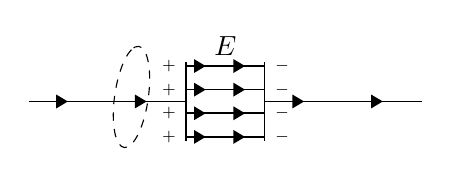
\begin{tikzpicture}[
		->-/.style = {decoration={markings,
				mark=between positions 0.25 and 0.75 step 0.5 with {\arrow{Triangle[scale=1]}}},
			postaction={decorate},
			semithick
		},]
		\draw[->-] (0,0.5,0) -- (2,0.5,0);
		\draw (2,0,0) -- (2,1,0);
		\draw (3,0,0) -- (3,1,0);
		\node at (2.5,1.2,0) {$E$};
		\foreach \y in {0.95, 0.65, 0.35, 0.05}
		{
			\node[anchor=east] at (2,\y,0) {\tiny$+$};
			\node[anchor=west] at (3,\y,0) {\tiny$-$};
			\draw[->-] (2,\y,0) -- (3,\y,0);
		};
		\draw[->-] (3,0.5,0) -- (5,0.5,0);
		\begin{scope}[canvas is yz plane at x=1.5]
			\draw[dashed] (0.75,0.5) circle (0.6);
			
		\end{scope}
	\end{tikzpicture}
	\caption{}
	\label{BADampere}
\end{figure}
\begin{figure}[b]
	\centering
	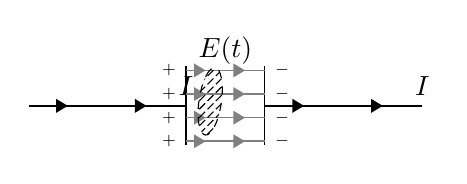
\begin{tikzpicture}[
		->-/.style = {decoration={markings,
				mark=between positions 0.25 and 0.75 step 0.5 with {\arrow{Triangle[scale=1]}}},
			postaction={decorate},
			semithick
		},]
		\draw[->-] (0,0.5,0) -- (2,0.5,0) node[above, align=center] {$I$};
		\draw (2,0,0) -- (2,1,0);
		\draw (3,0,0) -- (3,1,0);
		\node at (2.5,1.2,0) {$E(t)$};
		\foreach \y in {0.95, 0.65, 0.35, 0.05}
		{
			\node[anchor=east] at (2,\y,0) {\tiny$+$};
			\node[anchor=west] at (3,\y,0) {\tiny$-$};
			\draw[->-,color=black!50] (2,\y,0) -- (3,\y,0);
		};
		\draw[->-] (3,0.5,0) -- (5,0.5,0) node[above, align=center] {$I$};
		\begin{scope}[canvas is yz plane at x=2.5]
			\filldraw[pattern={north east lines}, dashed] (0.75,0.5) circle (0.4);
		\end{scope}
	\end{tikzpicture}
	\caption{}
	\label{goodampere}
\end{figure}
Maxwell corrected Ampere's law so that it could be appplied to magnetodynamics. The reason we require a correction is that, if we consider a setup like in \ref{BADampere}, we are able to easily calculate the magnetic field due to Ampere's law. However if we were to extend the surface so that it intersects through the middle of the parallel plate capacitor, we find that $\vb{j} = 0$, thus $\vb{B}=0$. This is a contradiction and implies that we must correct Ampere's law.
\\\\
Consider an electric field due to a parallel plate capacitor. We will consider an amperian loop between the plates of the capacitor of radius $r$, as in figure \ref{goodampere}. The current density will still be $\vb{j} = 0$. However, we can write the electric field due to the parallel plate capacitor as,
\begin{equation}
	E = \frac{Q}{\epsilon_0 A}
\end{equation}
However, as there is a current, the charge will be changing. We can then write a \textbf{displacement current},
\begin{equation}
	\dv{Q}{t} = I_{\text{dis}} = \epsilon_0A\pdv{E}{t},
\end{equation}
thus for this problem, we can rewrite Ampere's law as,
\begin{equation}
	\oint \vb{B}\cdot\dd{\vb{l}} = \mu_0\int \epsilon_0 \pdv{E}{t}\cdot\dd{\vb{A}}.
\end{equation}
We can write this more generally, which gives Ampere's 4th equation,
\begin{equation}
	\oint_C \vb{B}\cdot \dd{\vb{l}} = \mu_0 \int_S \left(\vb{j} + \epsilon_0 \pdv{E}{t}\right)\cdot\dd{\vb{A}}.
\end{equation}

\section{Mutual inductance}
Let us consider a setup like in figure \ref{fig:mutualinductance}. An increasing current $I_1$ runs through loop one, producing an increasing magnetic field $\vb{B}_1$. There is then a flux through loop 2, $\phi_{21}$ which produces an EMF $\varepsilon_2$, and thus a current $I_2$ through loop 2. This phenomenon is known as \textit{mutual inductance}, which we can define as a quantity $M$. Let us link the flux through loop 2 to the current through loop 1,
\begin{equation}
	\phi_{21} = M_{21}I_2.
\end{equation}
For a changing current, we get,
\begin{equation}
	\varepsilon_2 = - \dv{\phi_{21}}{t} = -M_{21}\dv{I_1}{t}.
\end{equation}
We get a similar relation for the other loop,
\begin{equation}
	\varepsilon_1 = - \dv{\phi_{12}}{t} = -M_{12}\dv{I_2}{t}.
\end{equation}
We will show that the two mutual inductances are equal, such that $M_{21} = M_{12} = M$.
\begin{figure}
	\centering
	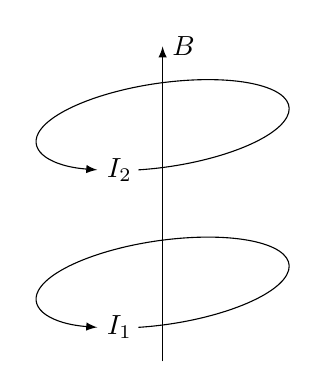
\begin{tikzpicture}
		\def\circledarrow#1#2#3#4{ % #1 Style, #2 Center, #3 Radius
			\draw[#1,->] (#2) +(80:#3) arc(80:-260:#3) node[anchor=west] {#4};
		}
		\draw[->] (0,1,0) -- (0,5,0) node[anchor=west] {$B$};
		\begin{scope}[canvas is xz plane at y = 2]
			\circledarrow{}{0,0}{1.5}{$I_1$};
		\end{scope}
		\begin{scope}[canvas is xz plane at y = 4]
			\circledarrow{}{0,0}{1.5}{$I_2$};
		\end{scope}
	\end{tikzpicture}
	\caption{Diagram showcasing mutual inductance}
	\label{fig:mutualinductance}
\end{figure}
\\\\
\subsection{Transformers}
Consider two coils wrapped around an iron core with $N_1$ and $N_2$ turns respectively. There will be a magnetic field $\vb{B}$ produced through the iron core. The flux through each turn is the same for each coil. We can say that the flux is directly proprotional to the number of turns,
\begin{align}
	\phi_1 \propto BN_1 && \phi_2 \propto BN_2 \\
	\implies && \frac{\phi_1}{\phi_2} = \frac{N_1}{N_2}.
\end{align}
A changing current implies,
\begin{equation}
	\dv{\phi_1}{t} = \frac{N_1}{N_2}\dv{\phi_2}{t}.
\end{equation}
By Faraday's law,
\begin{equation}
	\varepsilon_1 = \frac{N_1}{N_2}\varepsilon_2.
\end{equation}
Power is conserved, so,
\begin{equation}
	\varepsilon_1 I_1 = \varepsilon_2 I_2,
\end{equation}
so a transformer allows for AC voltage changes.
\subsection{Calculating mutual inductance}
Let us consider a solonoid. In the appendix, we calculated,
\begin{equation}
	B_1 = \mu_0 n_1 I_1 = \frac{\mu_0 N_1 I_1}{l}.
\end{equation}
For each turn, $\phi = B_1 A$, so,
\begin{equation}
	M = M_21 = \frac{\phi_2}{I_1} = \frac{N_2B_1A}{I_1}
\end{equation}
thus,
\begin{equation}
	M = \frac{\mu_0N_1N_2I_1A}{lI_1} = \frac{\mu_1N_1N_2A}{l}.
\end{equation}
\appendix
\chapter{Applied Examples}
\section{Rail Gun}
\begin{figure}[ht]
    \centering
    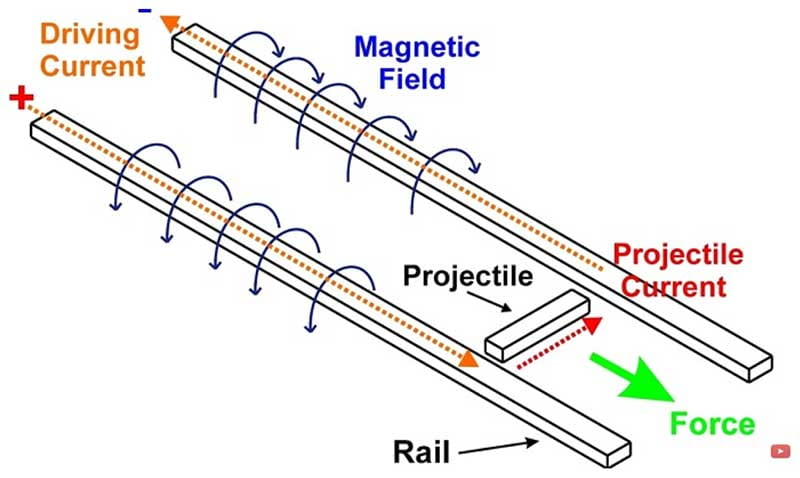
\includegraphics[width=200pt]{RailGunDiagram.jpg}
    \caption{Rail gun diagram.}
    \label{fig:railgun}
\end{figure}
\noindent
A railgun works by having two parallel beams and running an equal and opposite driving current through them. A projectile which is a conductor of length $l$ and mass $m$ is placed upon these beams, causing a current to run through it. There is a magnetic field "upwards", parallel to the beams. This will lead to a force to act on the on the projectile, of magnitude $F = BIl$, according to \eqref{forceonwire}. \\\\
The acceleration of the projectile will be given by Newton's second law, 
\begin{equation*}
    a = \frac{F}{m}.
\end{equation*}
We know that, if the length of the beams is $s$, the projectile's final velocity will be given by,
\begin{equation}
    \begin{split}
        v_{\text{final}} &= \sqrt{2as} \\
        & = \sqrt{\frac{2BIls}{m}}.
    \end{split}
\end{equation}
\section{Homopolar Generator}
\begin{figure}
    \centering
    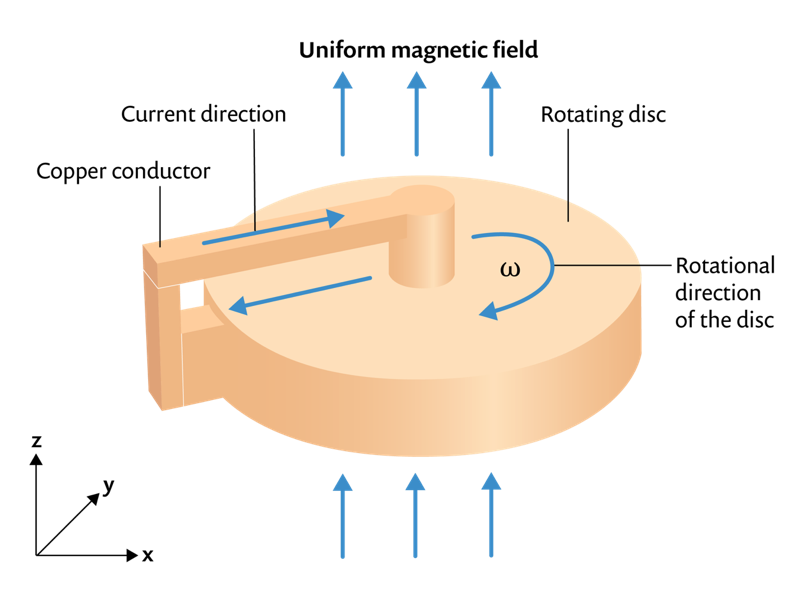
\includegraphics[width=200pt]{homopolar-generator-schematic.png}
    \caption{A diagram of a homopolar generator.}
    \label{fig:homopolar}
\end{figure}
This is an application of \textbf{Lenz's law}. Consider a setup like in figure \ref{fig:homopolar}. There is a disk of radius $a$ rotating perpendicular to a magnetic field $\vb{B}$ with an angular velocity $\omega$. We will consider a small segment of the disk from $r \to r + \dd{r}$. The velocity of the wheel is given by such that,
\begin{equation}
    \vb{v} = r\omega\vu*{\theta}.
\end{equation}
The force per unit charrge is given by \eqref{bfieldforce},
\begin{equation}
    \frac{1}{q}\vb{F} = \vb{v} \cross \vb{B} = vB\vu{r}.
\end{equation}
The infinitesimal potential difference from $r \to r + \dd{r}$ can be given by,
\begin{equation}
    (\vb{v}\cross\vb{B})\cdot\dd{l} = r\omega B\dd{r} 
\end{equation}
if we define $\dd{\vb{l}} = \dd{r}\vu{r}$. The total EMF created by the disk can then be given by,
\begin{equation}
    \varepsilon = \int_0^ar\omega B \dd{r} = \frac{1}{2}\omega B a^2.
\end{equation}

\chapter{Common Examples}
\section{Gauss' Law}
\section{Capacitors}
\subsection{Capacitance of parallel plate capacitor}
By Gauss' law, we know what the electric field due to an infinite plane of charge, by which the electric field of a parallell plate capacitor is,
\begin{equation}
    \vb{E} = \frac{Q}{\epsilon A}\vu{z}.
\end{equation}
Applying \eqref{potdiff} and by defining $\dd{\vb{l}} = \dd{z}\vu{z}$, we can obtain a potential,
\begin{equation}
    \Delta \phi = -\frac{Q}{\epsilon A}\int_d^0\dd{z} = \frac{Qd}{\epsilon_0 A}.
\end{equation}
By applying \eqref{capacitance},
\begin{equation}
    C = \frac{\epsilon_0A}{d}.
\end{equation}
\subsection{Capacitance of a cylindrical capacitor}
By Gauss' law, we know the charge due to a cylinder is,
\begin{equation}
    \vb{E} = \frac{\lambda}{2\pi r \epsilon_0}\vu{r}.
\end{equation}
Applying \eqref{potdiff} and by defining $\dd{\vb{l}} = \dd{r}\vu{r}$, we get,
\begin{equation}
    \Delta \phi = \frac{\lambda}{2\pi\epsilon_0}\ln{\frac{r_b}{r_a}}.
\end{equation}
By \eqref{capacitance}, we can define capacitance per unit length,
\begin{equation}
    \frac{C}{l} = \frac{2\pi\epsilon_0}{\ln{\frac{r_b}{r_a}}}
\end{equation}
\subsection{Capacitance of a spherical capacitor}
By Gauss' law, the electric field due to a sphere of charge is,
\begin{equation}
    \vb{E} = \frac{q}{4\pi\epsilon_0r^2}\vu{r}.
\end{equation}
Applying \eqref{potdiff} and by defining $\dd{\vb{l}} = \dd{r}\vu{r}$, we get,
\begin{equation}
    \Delta \phi = \frac{q}{4\pi\epsilon_0}\left(\frac{1}{r_a} - \frac{1}{r_b}\right).
\end{equation}
By \eqref{capacitance}, we obtain a capacitance,
\begin{equation}
    C = \frac{4\pi\epsilon_0r_ar_b}{r_a - r_b}
\end{equation}
\subsection{Energy dissipated through a capacitor}
Let us charge a capacitor of capacitance $C$ with a charge $Q$, and then discharge it through a resistor of resistance $R$ for a time $T$. Let us recall the following relations,
\begin{align}
    I = \dv{Q}{t} && \Delta\phi = \frac{Q}{C} && \Delta\phi = IR
\end{align}
which allow us to define write the differential equation,
\begin{equation}
    \dv{Q}{t} = \frac{Q}{RC}
\end{equation}
which can be solved to obtain,
\begin{equation}
    \ln{Q} = \frac{1}{RC}t + c \implies Q = Q_0e^{\frac{1}{RC}t}.
\end{equation}
Substituting for $I$,
\begin{equation}
    I = I_0e^{\frac{1}{RC}t}.
\end{equation}
We know that the power $\dv{E}{t}$ dissipated through a resistor is $I^2R$, so,
\begin{equation}
    \dv{E}{t} = I_0^2Re^{\frac{2}{RC}t},
\end{equation}
which is a differential equation which can be solved within the limits of $0\to T$ in order to find the total energy dissipated,
\begin{equation}
    E = \int_0^T I_0^2Re^{\frac{2}{RC}t}\dd{t}.
\end{equation}
\section{Biot-Savart Law}
\subsection{Loop of current}
\begin{figure}[h]
    \centering
    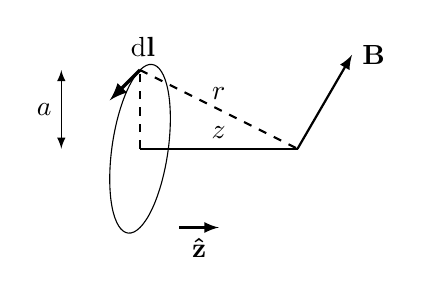
\begin{tikzpicture}
         \begin{scope}[canvas is yz plane at x=0]
            \draw (0,0) circle (1);
            \draw[dashed,thick] (0,0) -- (1,0);
            \draw[->, very thick] (1,0) -- (1,1) node[anchor=south,pos=-0.1] {$\dd{\vb{l}}$};
        \end{scope}
        \draw[dashed, thick] (0,1,0) -- (2,0,0)  node[above,midway] {$r$};
        \draw[thick] (0,0,0) -- (2,0,0) node[midway,above] {$z$};
        \draw[->,thick] (0.5,-1,0) -- (1,-1,0) node[midway,below] {$\vu{z}$};
        \draw[<->] (-1,0,0) -- (-1,1,0) node[anchor=east,midway] {$a$};
        \draw[->,thick] (2,0,0) -- (2.5,1,-0.5) node[anchor=west] {$\vb{B}$};
    \end{tikzpicture}
    \caption{Magnetic field due to loop of current.}
    \label{fig:loopof}
\end{figure}
\noindent
We will consider a loop $C$ of current $I$ and radius $a$. Let us define,
\begin{align}
    r^2 & = a^2 + z^2 & \cos\theta & = \frac{a}{r}.
\end{align}
Only components in the $\vu{z}$ direction are the ones which do not cancel. So, we can write,
\begin{equation}
    \dd{B_z} = \frac{\mu_0 I \dd{l}}{4\pi r^2} \cos\theta.
\end{equation}
Integrating,
\begin{equation}
\begin{split}
    B_z = \oint \frac{\mu_0 I}{4\pi r^2}\frac{a}{r}\dd{l} & = \frac{\mu_0 I a}{4\pi(a^2 + z^2)^{\frac{3}{2}}} \oint\dd{l} \\
    & = \frac{\mu_0 I a^2}{2(a^2 + z^2)^{\frac{3}{2}}}
\end{split}
\end{equation}
\subsection{Infinitely long wire}
\begin{figure}[h]
    \centering
    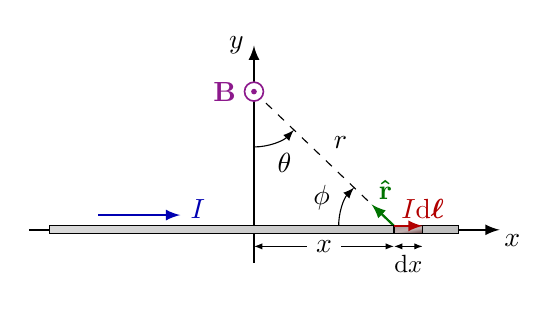
\begin{tikzpicture}
  \def\L{5.2}
  \def\W{0.10}
  \def\xmin{-0.55*\L}
  \def\xmax{0.6*\L}
  \def\ymin{-0.08*\L}
  \def\ymax{0.45*\L}
  \def\x{0.342*\L}
  \def\dx{0.07*\L}
  \coordinate (O) at (0,0);
  \coordinate (P) at (0,0.75*\ymax);
  \coordinate (X) at (\x,\W/2);
  
  % AXIS
  \draw[->,thick] (\xmin,0) -- (\xmax,0) node[below right=-2] {$x$};
  \draw[->,thick] (0,\ymin) -- (0,\ymax) node[left] {$y$};
  
  % MEASURES
  %\draw[<->] (0,0.2*\ymax) --++ (\x,0) node[midway,above] {$x$};
  \draw[measline] (    0,-0.09*\ymax) --++ (\x,0) node[measure] {$x$};
  \draw[measline] (   \x,-0.09*\ymax) --++ (\dx,0) node[midway,below,scale=0.9] {$\dd{x}$};
  %\draw[measline] (-\L/2,0.65*\ymin) --++ (\L,0) node[measure,right=10] {$L$};
  
  % POINT
  \node[Bcol,left=3] at (P) {$\vb{B}$};
  \draw[dashed] (P) -- (X) node[midway,above right] {$r$};
  \draw pic[->,"$\theta$",draw=black,angle radius=20,angle eccentricity=1.4] {angle = O--P--X};
  \draw pic[<-,"$\phi$",draw=black,angle radius=20,angle eccentricity=1.4] {angle = P--X--O};
  \draw[vector] (X) -- ($(X)!0.16!(P)$) node[right=5,above=-2] {$\vu{r}$};
  
  % VECTORS
  \draw[current] (-0.38*\L,0.08*\ymax) --++ (0.2*\L,0) node[above=2,right] {$I$};
  \pic at (P) {Bout}; %={fill=white}
  
  % ROD
  \draw[metal] (-\L/2,-\W/2) rectangle ++(\L,\W);
  \draw[darkmetal] (\x,-\W/2) rectangle ++(\dx,\W);
  %  node[midway,right=10,above=3] {$I\dd{x}$}; %I\dd{\ell}=
  \draw[force]
    (X) --++ (\dx,0) node[above=-1] {$I\!\dd{\vb*{\ell}}$};
  
\end{tikzpicture}
    \caption{Infinitely long wire}
    \label{fig:longwire}
\end{figure}\noindent
We are considering the setup in figure \ref{fig:longwire}, where the current through the wire produces a magnetic field which is a perpendicular distance $s$ away from the wire. Let us define,
\begin{align}
    r^2 & = z^2 + s^2 = \frac{s^2}{\cos^2\alpha} & \tan\alpha &= \frac{z}{s} & \dd{\vb{l}} = \dd{z}\vu{z}.
\end{align}
We can then find an expression for the magnetic field,
\begin{equation}
    \vb{B}_p = \frac{\mu_0 l }{4\pi} \int_C \frac{\vu{z}\cross\vu{r}}{r^2}\dd{z}.
\end{equation}
Since $\vu{z}$ and $\vu{r}$ are not parallel, so we can say,
\begin{equation}
    \vu{z}\cross\vu{r} = |\vu{z}||\vu{r}|\sin\beta\vu*{\theta} = \cos\alpha\vu*{\theta}.
\end{equation}
We must then rewrite our integral so that we are integrating over $\alpha$. We know,
\begin{equation}
    z = s\tan\alpha \implies \dd{z} = \frac{s\dd{\alpha}}{\cos^2\alpha}.
\end{equation}
We can now begin to find an expression for the magnetic field dependent on $s$,
\begin{equation}
    \vb{B}(s) = \frac{\mu_0 I}{4\pi}\int_C \frac{\cos\alpha}{\left(\dfrac{s^2}{\cos^2\alpha}\right)}\frac{s}{\cos^2\alpha}\dd{\alpha} = \frac{\mu_0 I}{4\pi} \vu*{\theta} \int_C \frac{\cos\alpha}{s}\dd{\alpha}.
\end{equation}
For an infinite wire, the limits of $\alpha$ are $-\frac{\pi}{2} \to +\frac{\pi}{2}$,
\begin{equation}
    \vb{B}(s) = \frac{\mu_0 I}{2\pi s}\vu*{\theta}.
\end{equation}
\begin{figure}
    \centering
    % WIRE B FIELD 3D
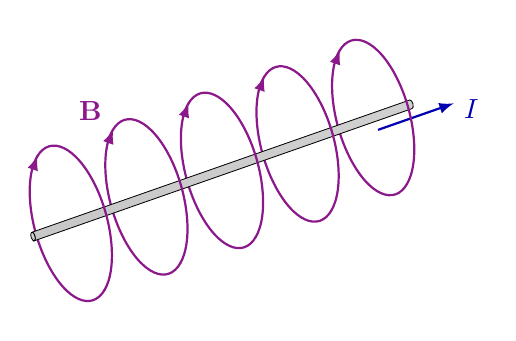
\begin{tikzpicture}[z={(0.8,0.28)},x={(0.58,-0.45)}]
  \def\L{6}
  \def\W{0.10}
  \def\R{0.9}
  \def\ang{-35}
  \def\scale{1.3}
  \def\NB{5}
  \coordinate (O) at (0,0,0);
  %\draw (0,0,0) -- (2,0,0);
  %\draw (0,0,0) -- (0,0,2);
  
  % B FIELD BACK
  \foreach \i [evaluate={\x=(\i-\NB/2-0.5)*\L/\NB;}] in {1,...,\NB}{
    %\draw[BField,-] (0,0,\x)++(\ang+1:\R) arc (\ang+1:\ang-181:\R);
    \draw[BFieldLine=1] (0,0,\x)++(\ang+1:\R) arc (\ang+1:\ang-181:\R) --++ (65:0.001*\R);
  }
  
  % WIRE
  \draw[metal] (0,0,-\L/2)++(120:\W/2) --++ (0,0,\L) arc (120:-60:\W/2) --++ (0,0,-\L) arc (-60:120:\W/2);
  \draw[metal] (0,0,-\L/2) circle (\W/2);
  \draw[current] (0.12*\R,-0.12*\R,0.4*\L) --++ (0,0,0.2*\L) node[below=2,right] {$I$};
  
  % B FIELD FRONT
  \foreach \i [evaluate={\x=(\i-\NB/2-0.5)*\L/\NB;}] in {1,...,\NB}{
    %\draw[BFieldLine=1] (0,0,\x)++(\ang+180:\R) arc (\ang+180:\ang:\R) --++ (-116:0.001*\R);
    \draw[BField,-] (0,0,\x)++(\ang+180:\R) arc (\ang+180:\ang:\R);
  }
  \node[Bcol] at (-0.9*\R,0.9*\R,-0.25*\L) {$\vb{B}$}; %++(140:1.3*\R)
  
\end{tikzpicture}
    \caption{Magnetic field due to infinitely long wire.}
    \label{fig:enter-label}
\end{figure}
\subsubsection{Forces on current carrying wires.}
The force per unit length for current carrying wires is then given by,
\begin{equation}
    \frac{F}{l} = \frac{\mu_0 I_1I_2}{2\pi s}.
\end{equation}
The proof is trivial. For current travelling in the same direction, the force is attractive, and vice versa.
\section{Ampere's Law}
\subsection{Solenoids}
\begin{figure}
    \centering
    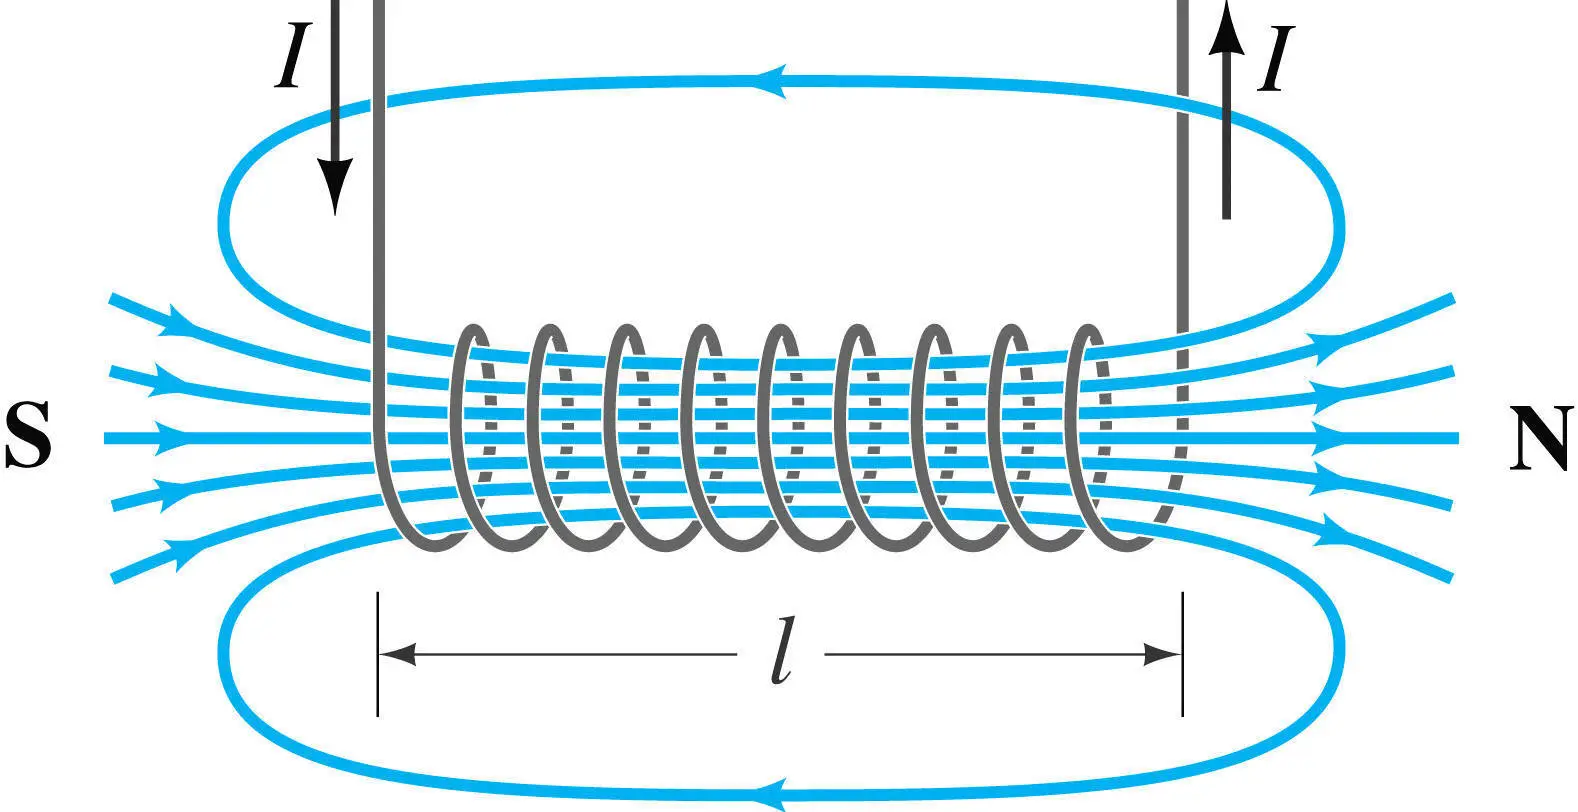
\includegraphics[width=200pt]{solenoid-magnetic-field.png}
    \caption{Solonoid}
    \label{fig:solonoid}
\end{figure}
A solenoid is a helical coil with $N$ turns and length $l$ such that the turns per unit length are given by $n = \frac{N}{l}$. \\\\
We are interested in the electric field inside the solenoid. We know that each loop will create a magnetic field which will superimpose with all other magnetic fields, such that the magnetic field is approximately uniform inside the coil and approximately 0 outside. 
\\\\
Let us consider a setup like in figure \ref{fig:solonoid}. There is a rectangular Amperian loop $C$ of length $l$. We can state that the total circulation of the magnetic field is,
\begin{equation}
    \oint \vb{B}\cdot\dd{\vb{l}} = \int_{a\to b} \vb{B}\cdot\dd{\vb{l}} + \int_{b\to c} \vb{B}\cdot\dd{\vb{l}} + \int_{c\to d} \vb{B}\cdot\dd{\vb{l}} + \int_{d\to c} \vb{B}\cdot\dd{\vb{l}}.
\end{equation}
Let us consider each region. From $a\to b$ the Amperian loop passes parallel through the magnetic field, such that,
\begin{equation}
    \int_{a\to b}\vb{B}\cdot\dd{\vb{l}} = B_{\text{in}}l.
\end{equation}
For $b\to c$ and $c \to d$, the loop is perpendicular to the magnetic field, so the circulation is equal to 0. For $d \to a$ the loop passes through no magnetic field, so the circulation is 0. Thus, we can conclude, for a coil where $nl$ coils are carrying a current $I$
\begin{equation}
    \oint_C \vb{B}\cdot \dd{\vb{l}} = \mu_0 I_{\text{enc}} = \mu_0 nlI,
\end{equation}
and thus the magnitude of the magnetic field is,
\begin{equation}
    B_{\text{in}} = \mu_0 n I.
\end{equation}
\section{Faraday's Law}
\subsection{Loop of wire through magnetic field}
\begin{figure}
	\centering
	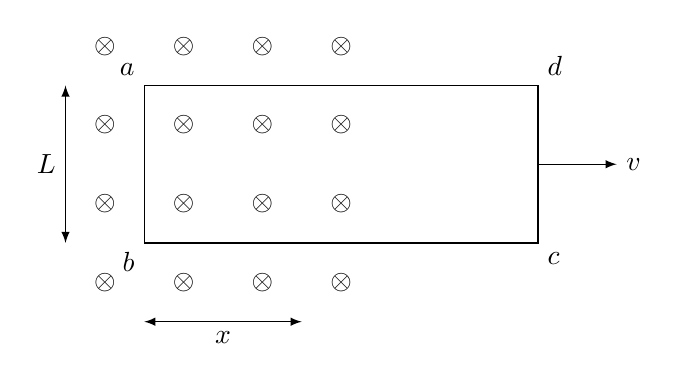
\begin{tikzpicture}
		\foreach \i in {1,2,3,4}
		{
			\node at (\i,\i) {$\otimes$};
		}
		
		\foreach \i in {2,3,4}
		{
			\node at (\i, 1) {$\otimes$};
			\node at (1, \i) {$\otimes$};
		}
		\node at (3,2) {$\otimes$};
		\node at (4,2) {$\otimes$};
		\node at (4,3) {$\otimes$};
		\node at (2,3) {$\otimes$};
		\node at (2,4) {$\otimes$};
		\node at (3,4) {$\otimes$};
		\draw (1.5,1.5) rectangle (6.5,3.5);
		\node[anchor=south east] at (1.5,3.5) {$a$}; 
		\node[anchor=north east] at (1.5,1.5) {$b$};
		\node[anchor=north west] at (6.5,1.5) {$c$};
		\node[anchor=south west] at (6.5,3.5) {$d$};
		\draw[->] (6.5,2.5) -- (7.5,2.5) node[anchor=west] {$v$};
		\draw[<->] (0.5,1.5) -- (0.5,3.5);
		\node[anchor=east] at (0.5,2.5) {$L$};
		\draw[<->] (1.5,0.5) -- (3.5,0.5);
		\node[anchor = north] at (2.5,0.5) {$x$}; 
	\end{tikzpicture}
	\caption{A loop of wire partially through a magnetic field.}
	\label{loopofwire}
\end{figure}
Consider a setup like in \ref{loopofwire}. If we consider an electron moving from $a \to b$ like in figure \ref{electronmotion}.  By \eqref{bfieldforce}, the electron experiences a downard force and moves downards. An electron going from $b \to c$ also experiences a downards force, but is constrained in the wire so it cannot move in the vertical direction. Similarly for $d \to a$. Electrons in $c \to d$ are not present in the magnetic field so experience no force.
\\\\
Because there is an excess of charge carriers in one part of the loop, electrons must move in an anti-clockwise motion around the loop, producing a current in a clockwise direction. 
\\\\
We can obtain an equation for $\varepsilon$ by considering \eqref{emf}. Trivially, $\int\vb{B}\cdot\dd{\vb{A}} = BLx$. Taking the time derivative, $BL\dv{}{t}\left(x\right) = Blv$.
\begin{figure}
	\centering
	\begin{tikzpicture}
		\draw (0,0) -- (0,3);
		\node at (0,1.5) {\textbullet};
		\node[anchor=east] at (0,1.5) {$e^-$};
		\draw[->] (0.25,1.5) -- (0.25,0.7) node[anchor=west] {$\vb{F}$};
		\draw[->] (0,2.5) -- (1,2.5) node[anchor=west] {$\vb{v}$};
		\node at (2,1) {$\otimes$ $\vb{B}$}; 
	\end{tikzpicture}
	\caption{}
	\label{electronmotion}
\end{figure}
\chapter{Maxwell's Laws}
Here are given Maxwell's 4 laws in integral form:
\begin{align}
	&\oint \vb{E}\cdot\dd{\vb{A}} = \frac{Q_{\text{enc}}}{\epsilon_0} \\
	&\oint_S \vb{B}\cdot\dd{\vb{A}} = 0 \\
	&\oint_C \vb{E}\cdot\dd{\vb{l}} = -\dv{}{t}\int\vb{B}\cdot\dd{\vb{A}} \\
	&\oint_C\vb{B}\cdot\dd{\vb{l}} = \mu_0\int_S\left(\vb{j} + \epsilon_0\pdv{\vb{E}}{t}\right)\cdot \dd{\vb{A}}
\end{align}
\end{document}
